\documentclass[twocolumn]{IEEEtran}
\usepackage{amsmath}
\usepackage{graphics}
\usepackage{graphicx}
\usepackage[english]{babel}

\bibliographystyle{/home/rsheissa/papers/iced_2006/ieeebib}

%\pagestyle{empty}

\begin{document}
%\thispagestyle{empty}
\title{Automated CAD Tools for Design of Nullor-based Amplifiers}

\author{Roberto Casta\~neda-Sheissa, Arturo Sarmiento-Reyes, Luis Hern\'andez-Mart\'inez\\ National Institute for Astrophysics, Optics and Electronics\\
Electronics Department, CAD Group\\ P.O. Box 51, 72000, Puebla, Pue., Mexico}

\maketitle
\thispagestyle{empty}
\pagestyle{empty}
\begin{abstract}
Computer aided design (CAD) tools are aimed to speed-up processes, simplify calculations and perform complex tasks with minimum effort. CAD tools are present in many fields like chemistry, physiscs, mathematics, astrophysics, engineering and electronics. For electronics, CAD tools are developed mainly to perform verification tasks and, because the complexity it implies, there is a lack of electronic design tools. By means of a design methodology known as Structured Design, it is possible to develop a CAD tool. This work represents the development of a CAD tool for automated design of amplifiers based on the guidelines provided by Structured Design and programmed in C++.
\end{abstract}

\section{Introduction}
The production of any electronic circuit is concerned with successively taking a requirement; developing it; producing an accurate abstract representation (a circuit diagram); making, evaluating, and testing it; and then returning to the original circuit design to correct errors. This process is iterative, frequently extending across the lifetime of the circuit, with modifications and improvements introduced and specifications changed continuously. This way to perform a development involves the construction and manipulation of various (often large) representations of a circuit and the examination and testing of these with respect to the initial requirements. The development of any sub-circuit representation for running a test can be long and complicated. Performing a complete set of these design activities for a system of any size is long and, specially, costly. The computer's ability to contain large amounts of data and to facilitate its access and updating in a dynamic way, together of course with powerful programs for aiding in the synthesis and analysis of circuits, is a major for their use.

With each new level of refinement, more information concerned with the detailed physical and functional implementation of their circuit is included in the description. The design process involves transformation between these represenatations during both synthesis and verification. There are many programs designed to produce one representation of the design process and the output given to another tool for further post-processing. However for many of these tasks, programs are not perfect and much human intervention is still needed. For large designs, this is very expensive because more than one product iteration is frequently required to remove all errors before a working design is produced.

The term CAD {\it framework} has come to mean all of the underlying facilities provided to the CAD tool {\it developer}, the CAD system {\it integrator}, and the {\it end user} (IC or system designer) which are necessary to facilitate their tasks.

Broadly speaking, these three groups of people represent the user of the CAD framework, each with their own needs and particular emphasis. The CAD framework plays an analogous role in the development of engineering-specific, or even electrical-engineering-specific, software systems to the role played by an operating system for the development of general-purpose software applications, or the role of a specific programming environment for software development in a particular programming language \cite{barnes}. 
\section{Electronic Structured Design}
Electronic circuit design consists on a search through many combinations with several kind of components and different kind of properties. It would be a great time investment to find an apt circuit by means of extensive tests with every possible combination of available components. Therefore it is necessary to stablish a strategy to find the right solution as soon as possible. The most common strategy for circuit design is to use certain circuit topology, then by changing some parameters within the circuit a solution that fulfils the requirements of the designer is found \cite{verhoeven}. The way that this new design behaves within certain constraints, is going to stablish the validity of it. In case that the design is not useful, the design process is restarted. Even though that this strategy provides valid results sooner or later, there are serious disadvantages on it:

\begin{itemize}
\item There is no guarantee that the found solution is the {\it optimum} and does not provide any information on how close it is.
\item Relationship between component parameters and circuit performance is never explicit. Incidentally, circuit performance can be sensitive for certain irrelevant parameter because the circuit is not suitable for the application.
\item It is really complicated to determine what it should be changed in a circuit when, for instance, constraints are changed.
\end{itemize}

To create order from the chaos that the electronic amplifier design is, design is separated in smaller problems, all orthogonal if possible, which allows to clarify the problem and makes easier the solution process. {\it Structured electronic design} \cite{verhoeven,nordholt} is a method that allows find just {\bf ONE} solution to the design problem in a quick way. Nevertheless this is a method based on certain amount of suppositions and a limited amount of rules. Therefore, the practical application of the electronic structured design should never, and by any means, create a dogmatic reject for the given results by the traditional design strategy or any other strategy provided that this would incite a delay on the evolution of the design strategy.

Amplifier structured design focuses on three fundamental aspects in order to provide the description on how the circuit behaves:

\begin{itemize}
\item Noise.
\item Distortion.
\item Bandwidth.
\end{itemize}

In order to accelerate the design process, several suppositions should be established as stated previously. These will be enforced based on the basic specs that should be provided, on the circuit behaviour given the results by employing simpler models and to the decisions concerning \mbox{every} stage of the design in particular. This kind of design is based on the following basic elements:

\begin{itemize}
\item Orthogonality - Circuits should be order in such a way that the behaviour of the the three fundamental aspects can be designed orthogonally, that is, the behaviour of a stage should not have any influence on the other two.
\item Simplicity - Simple models are defined to obtain quick predictions on the feasibility of the circuit. Non feasible solutions can be detected on the first stages of the design. Special planning should be done in order to stablish that the estimated results are as close as possible to the real ones.
\item Hierarchy - Design hierarchy allows to reduce the complexity of the design problem because allows its efficient division in smaller and independent design problems. Planning at this point should be arranged in such a way that decisions taken on a certain hierarchical level are kept valid throughout the rest of the design.
\end{itemize}

\section{CAD Tool Structure}
Given the basic blocks that structured design is based on to create an amplifier, a rather general structure for the design based on these blocks is shown in Figure \ref{fig:descad}. This tool has been developed under the code name {\it Descad\_Wizard} to reflect that the adequate way to operate this tool is using a {\it wizard} approach, that is, development process is performed by filling up some options within a window. Calculations are programmed in C++ \cite{joyanes} and the graphical user interface is provided by Qt \cite{qt}. 

\begin{figure}[hbtp]
	\centering
	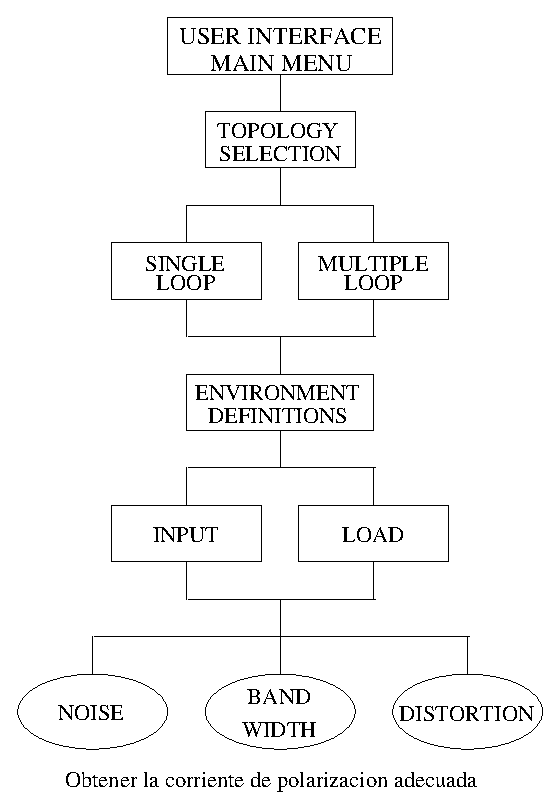
\includegraphics[scale=0.5]{figuras/DESCAD_1.eps}
	\caption{General structure for the CAD tool.}
	\label{fig:descad}
\end{figure}

Figure \ref{fig:des1} shows the first window where basic specifications are typed. Basic requirements refers to the basic amplifier structure like:

\begin{itemize}
\item Amplifier types.
\item Amplifier configuration.
\item Source and load types and values.
\item Gain and sign specs.
\end{itemize}

\begin{figure}[hbtp]
	\centering
	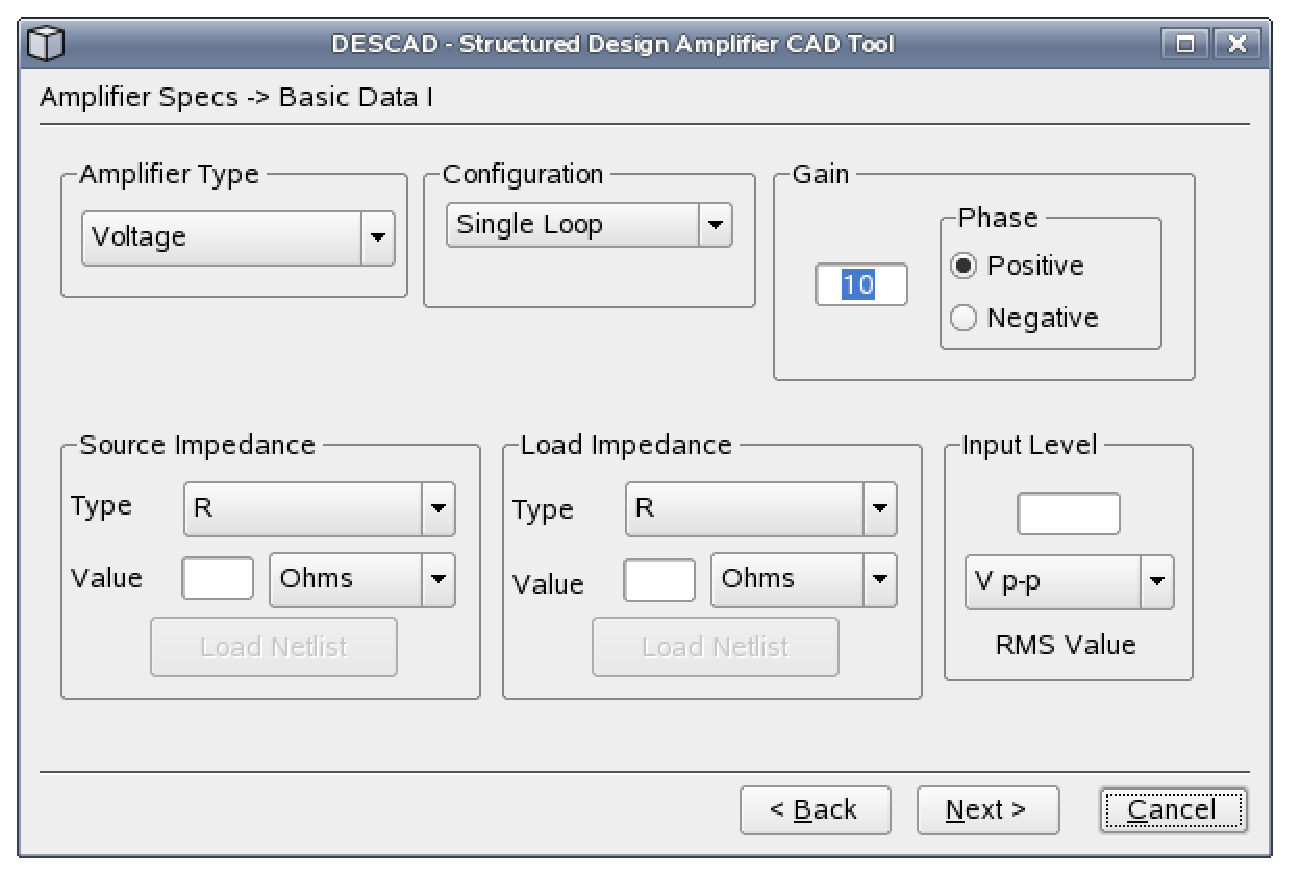
\includegraphics[scale=0.3]{figuras/step1.eps}
	\caption{Basic specifications window.}
	\label{fig:des1}
\end{figure}

The gain value can be provided as a floating-point number or in scientific format; phase value refers to the output phase that is desired at the output port of the amplifier. Phase can be positive (no phase change) or negative (phase is shifted $180\,^{\circ}$ away). Another specification to be provided is the desired configuration, it could be one of two options. First option is to select one of the single-loop amplifiers: (1) voltage amplifier, (2) transconductance amplifier, (3) transresistance amplifier and (4) current amplifier. These amplifiers are depicted in Figure \ref{fig:amps}. Second option is a two-loop amplifier. This type of amplifier comprises the transconductance and transresistance amplifiers. Figure \ref{fig:two_loop}.

\begin{figure}[hbtp]
	\centering
	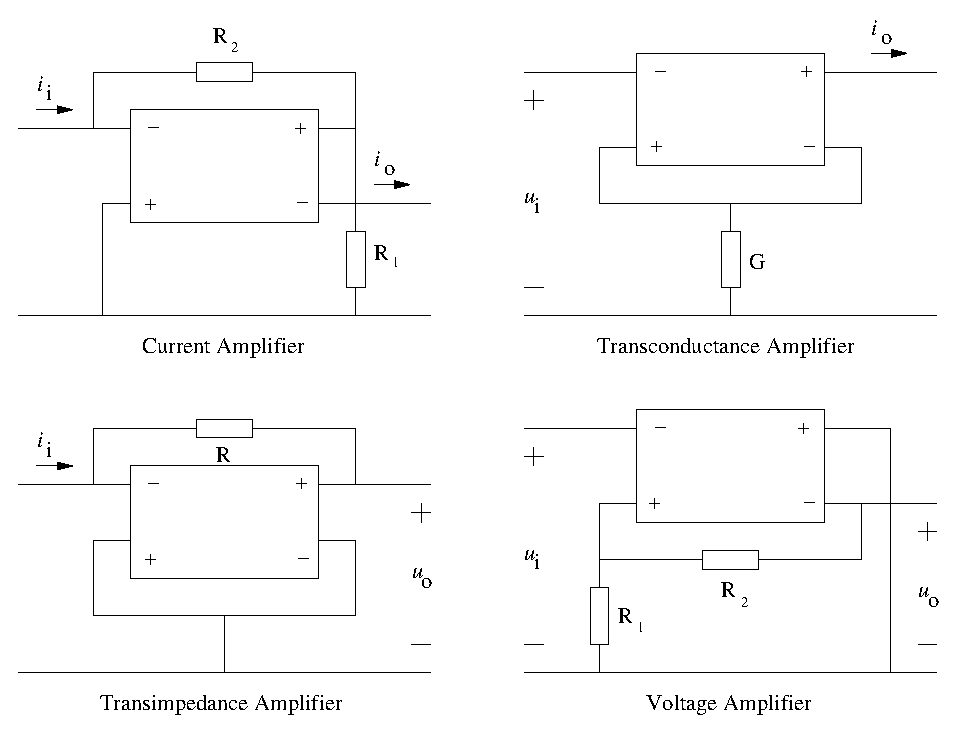
\includegraphics[scale=0.5]{figuras/grupo_eng.eps}
	\caption{Amplifier types.}
	\label{fig:amps}
\end{figure}

\begin{figure}[hbtp]
	\centering
	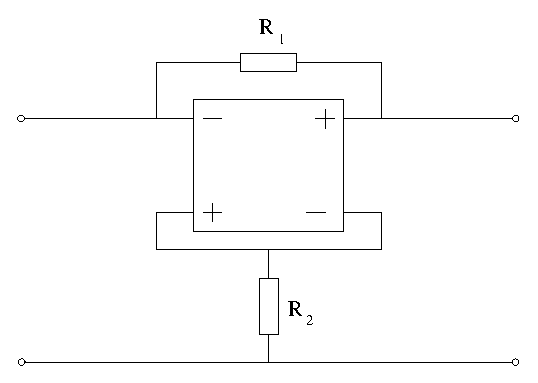
\includegraphics[scale=0.5]{figuras/twoloop_basica.eps}
	\caption{Two-loop amplifier topology.}
	\label{fig:two_loop}
\end{figure}

For the synthesis of noise, clipping and bandwidth stages a scheme is provided in Figure \ref{fig:descad2}. It means that for every stage it is possible to choose a single device or differential (two devices) configurations; it is worth noting that in order to keep the negative feedback behaviour a differential configuration must be placed either on noise or clipping stages. Windows for the noise and clipping stages are depicted in Figure \ref{fig:descad3} and Figure \ref{fig:descad4}.

\begin{figure}[hbtp]
	\centering
	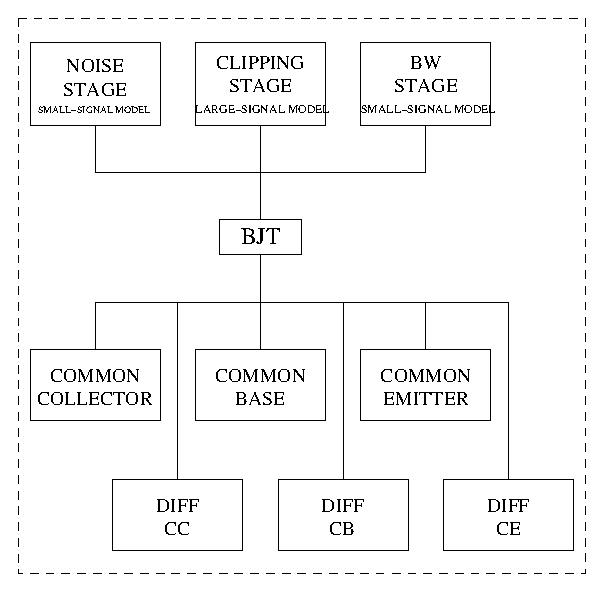
\includegraphics[scale=0.5]{figuras/descad2.eps}
	\caption{Noise, clipping and bandwidth synthesis scheme.}
	\label{fig:descad2}
\end{figure}

\begin{figure}[hbtp]
	\centering
	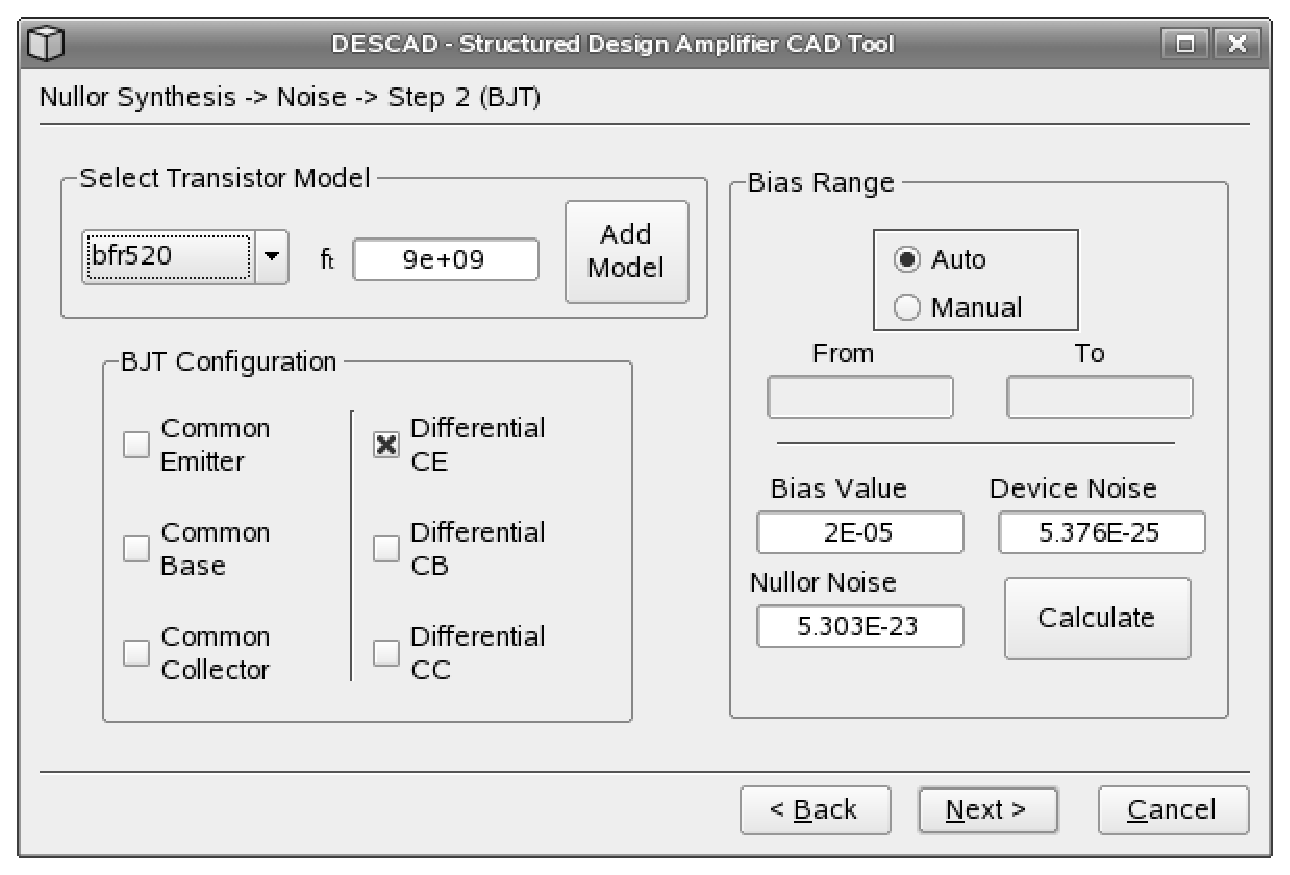
\includegraphics[scale=0.3]{figuras/wizard3.eps}
	\caption{Noise stage window.}
	\label{fig:descad3}
\end{figure}

\begin{figure}[hbtp]
	\centering
	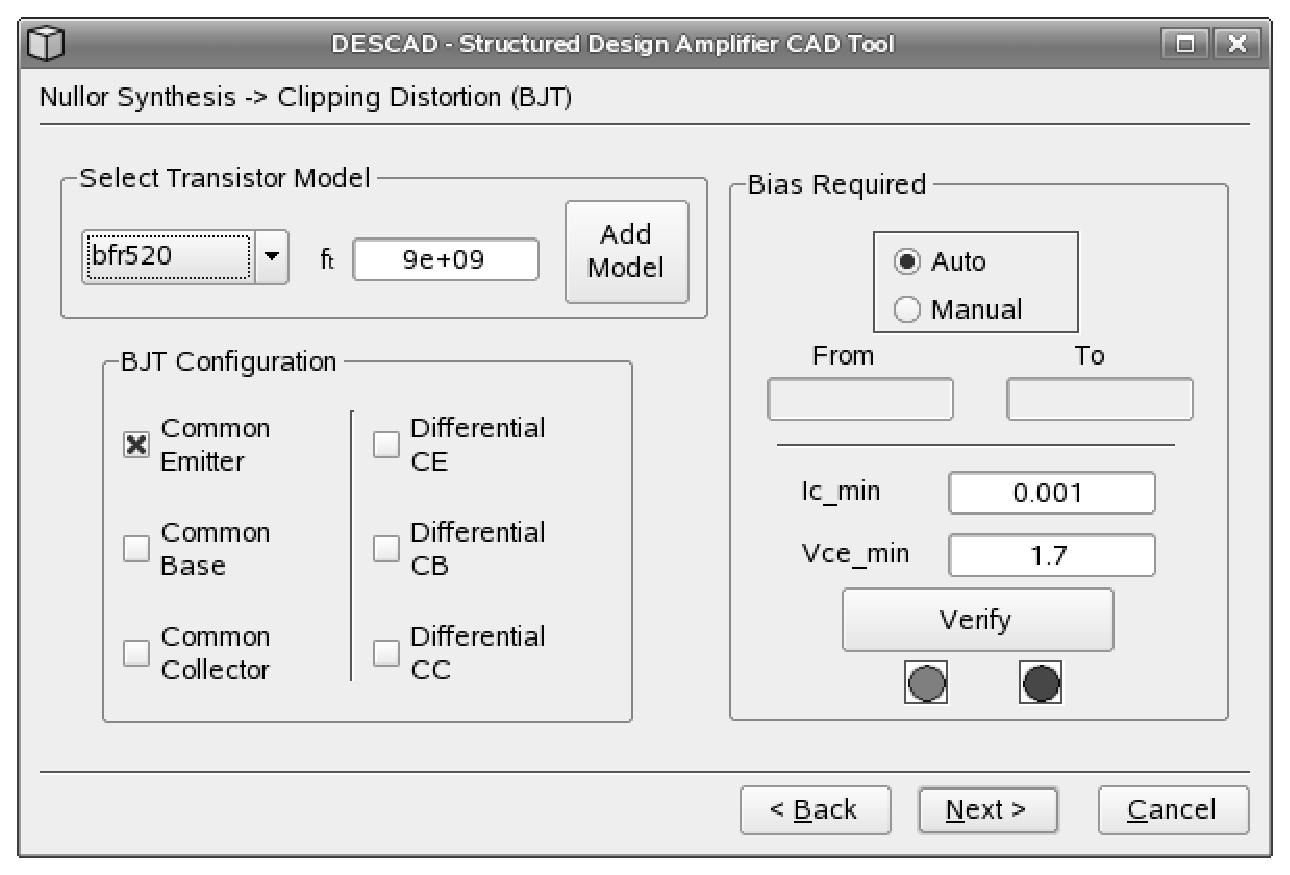
\includegraphics[scale=0.3]{figuras/wizard4.eps}
	\caption{Clipping stage window.}
	\label{fig:descad4}
\end{figure}

Bandwidth synthesis process is divided in two steps: (1) calculate the LP-product \cite{verhoeven} in order to verify if design is capable to handle the desire bandwidth and (2) in order to guarantee a flat output frequency response, amplifier poles must be located at Butterworth locations \cite{nordholt}. In case that the LP-product is not high enough for the desired bandwidth, there are three options to be applied in this order: (1) increase collector current for the noise stage as high as the noise behaviour is kept within constraints. (2) If the LP-product is still low, an increase on the collector current for the clipping stage is performed. This increase can only be applied if clipping is below the allowed value. (3) Last case is to add another device to the design increasing the amplifier degree by 1. Figure \ref{fig:descad5} shows the LP-product window.

\begin{figure}[hbtp]
	\centering
	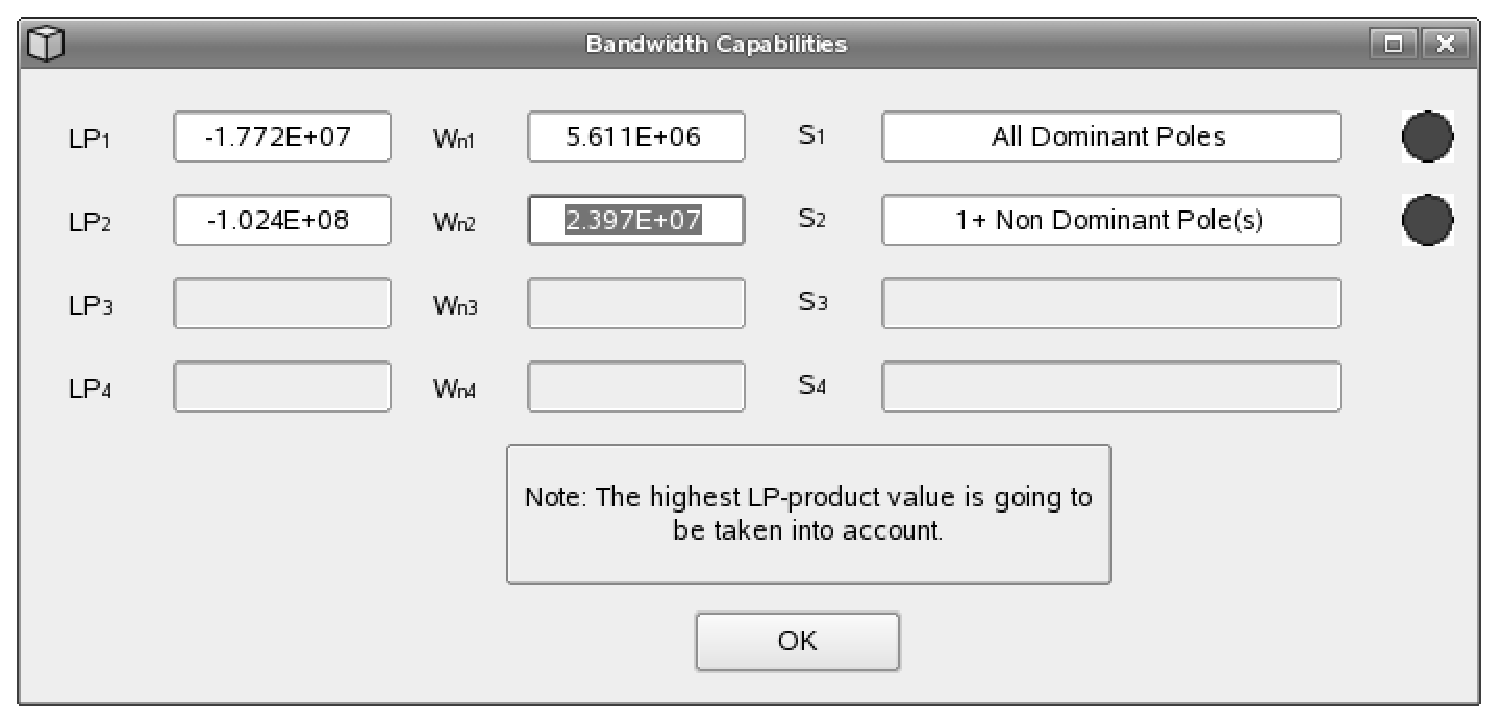
\includegraphics[scale=0.3]{figuras/wizard5.eps}
	\caption{The LP-product window.}
	\label{fig:descad5}
\end{figure}

Once the LP-product is high enough the process to place the closed-loop poles of the amplifier in Butterworth position is performed. \cite{verhoeven} and \cite{nordholt} provide the adequate compensation techniques in order to place the amplifier poles at the required location. Given the fact that it is possible to perform compensation at the input port, output port and feedback network the user is capable to select where to perform the compensation. Nevertheless if compensation fails to adjust the poles position, a warning message is displayed and the option is disabled then the user must select any available option. Figure \ref{fig:descad6}.

\begin{figure}[hbtp]
	\centering
	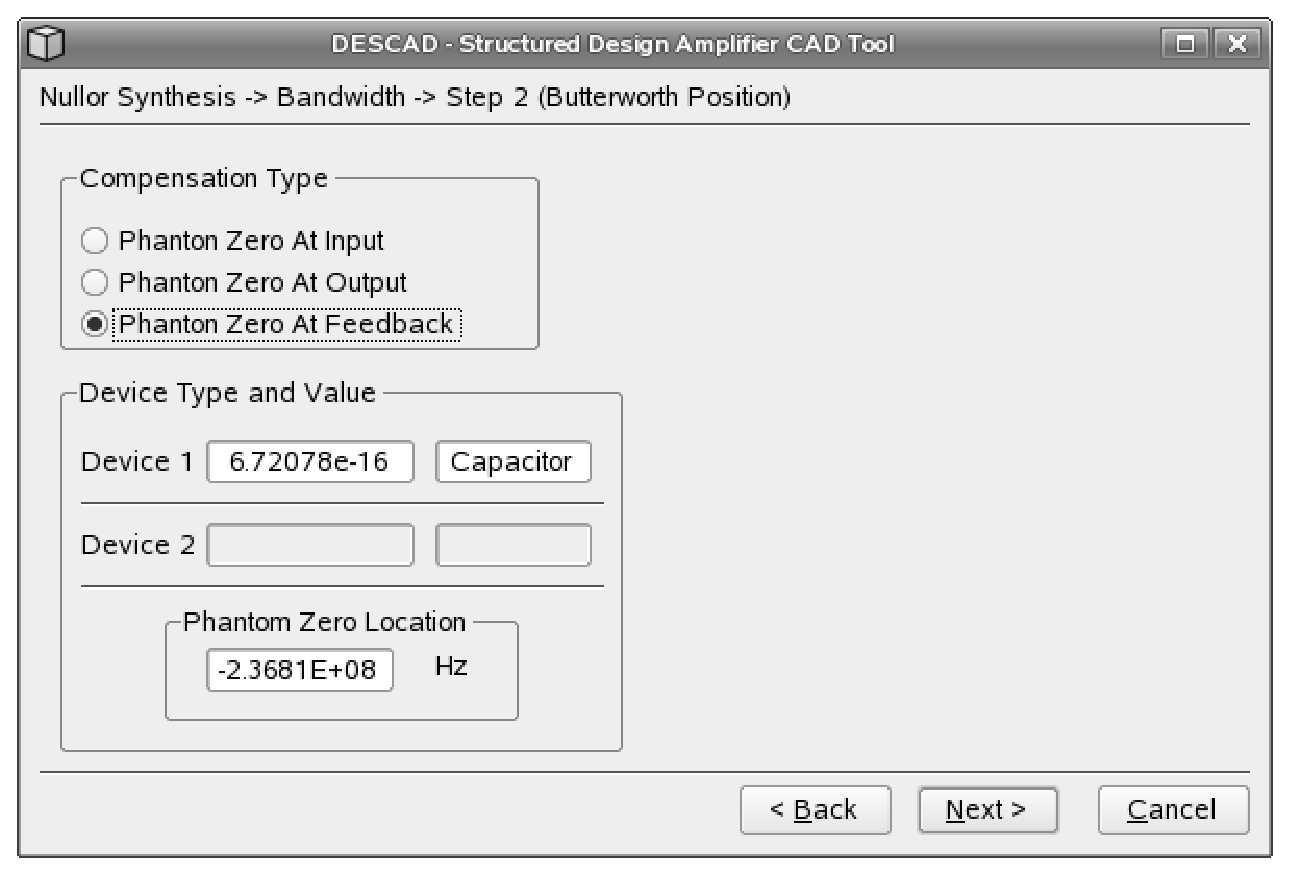
\includegraphics[scale=0.3]{figuras/wizard6.eps}
	\caption{Butterworth compensation stage.}
	\label{fig:descad6}
\end{figure}

Finally a summary is displayed providing the constraints given by the user and the results of the synthesis procedure. Besides an input file for an industrial simulator is generated. Figure \ref{fig:descad7}.

\begin{figure}[hbtp]
	\centering
	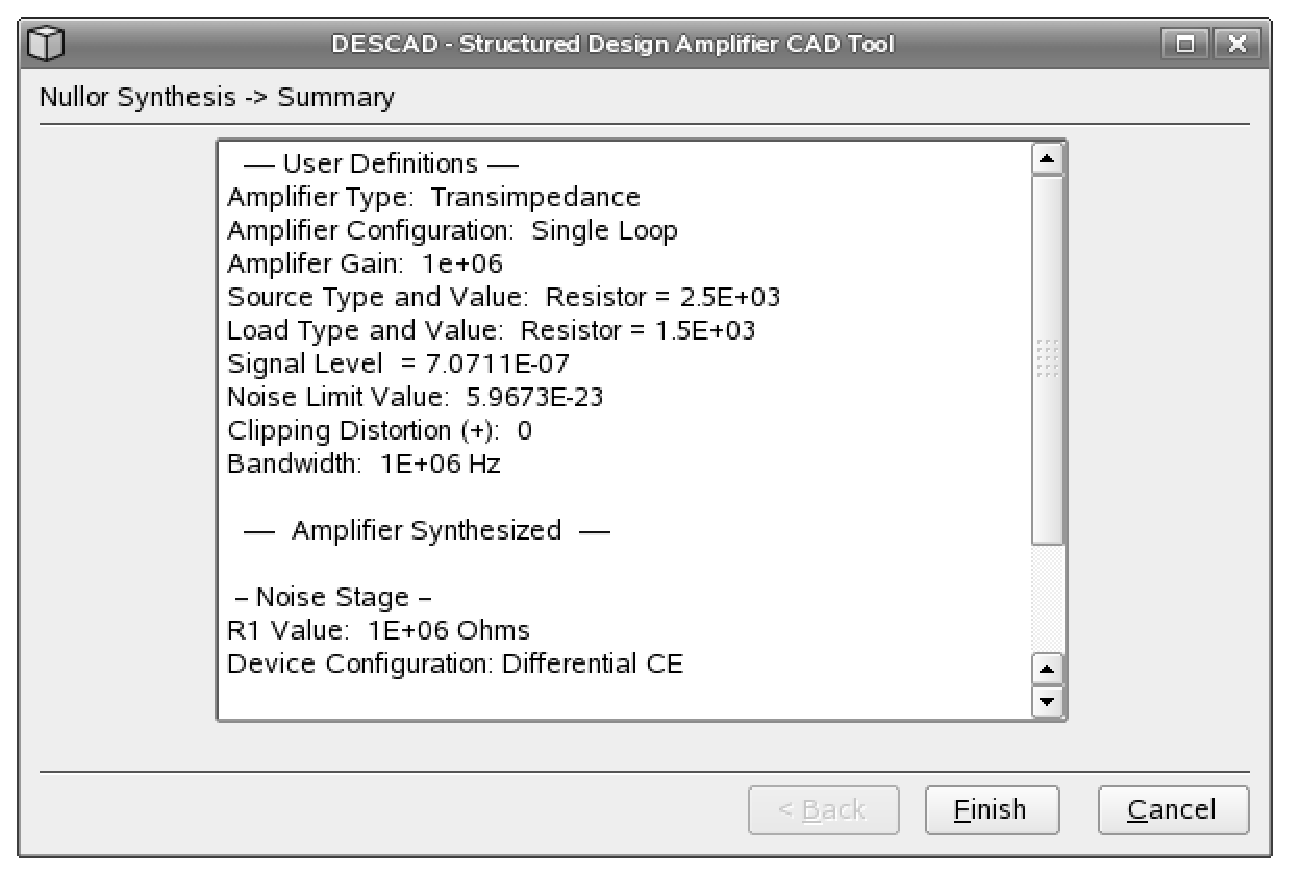
\includegraphics[scale=0.3]{figuras/wizard8.eps}
	\caption{Design summary window.}
	\label{fig:descad7}
\end{figure}

\section{Example}
As an example a transconductance amplifier is going to be designed and must satisfy these constraints:

\begin{itemize}
\item Source Type and Value: Resistor - $5K{\Omega}$
\item Load Type and Value: Resistor - $1.5K{\Omega}$
\item Input Level: .5 $\mu$A
\item Output Level: .5 V
\item Noise Level: 10 dB
\item Clipping: 0 \%
\item Bandwidth: 1 MHz
\end{itemize}

Noise values calculated for the feedback and source impedances:

\begin{itemize}
\item Source Noise: 3.315E-24 $A^2/Hz$
\item Feedback Noise: 1.658E-26 $A^2/Hz$
\end{itemize}

The nullor synthesis for the noise stage is performed with the transistor BFR520 \cite{bfr520} in differential common emitter configuration. The minimum $I_C$ and noise values are: 

\begin{itemize}
\item $I_C=2E-5\;A$
\item Noise=1.351E-25 $A^2/Hz$
\end{itemize}

Clipping distortion stage synthesis is provided by the transistor BFR520 in common emitter configuration. Values are:

\begin{itemize}
\item $I_C=0.001\;A$
\item $V_{CE}=1.7$ V
\end{itemize}

Note that values on the clipping stage are compared to the maximum allowable values taken from the device datasheet. For the bandwidth stage and the LP-product calculation process on the first run the result was that the LP-product is high enough but had one or more non dominant poles. This behaviour is not desired because affects the overall gain, consequently an adjustment is required. The adjustment is performed on the noise stage because it has the best $I_C$ range. Consequently the new values for the noise stage are:

\begin{itemize}
\item $I_C=0.001\;A$
\item Noise=3.226E-26 $A^2/Hz$
\end{itemize}

Hence for the Butterworth compensation process it is performed at the feedback network. In this case a capacitor is placed in parallel to the feedback resistor and its value is $C=9.50872E-16$F.

Simulation on the amplifier circuit is performed using HSpice \cite{hspice}. Instead of using the actual active device, \mbox{small-signal} elements are employed. Small-signal values are calculated using the $I_C$ found for each synthesised stage. Figure \ref{fig:sim} shows the resulting. As it can be seen a flat output behaviour is achieved on the desired frequency.

\begin{figure}[hbtp]
	\centering
	\includegraphics[scale=0.3,angle=-90]{figuras/iced_2006.ps}
	\caption{Amplifier simulation output.}
	\label{fig:sim}
\end{figure}

\section{Conclusions}
An automated design tool for nullor-based amplifiers has been presented. Based on the {\it Structured Design} methodology and with the aid of the C++ programming language, this CAD tool is capable to speed-up the design process. A {\it wizard} driven tool helps the user to make easier decisions and concentrate only on certain aspects of the design while calculations are performed without user intervention. Results given by the tool can be simulated for verification purposes using the small-signal equivalent of their components. Consequently simulation can be performed directly on the AC domain without the worry about DC concerns.

\bibliography{bib/iced2006}
\end{document}
